\documentclass[leqno]{article}
\usepackage{verbatim}
\usepackage{array}
\usepackage{listings}
\usepackage{fancyvrb}
\usepackage{enumitem}

\usepackage[utf8]{inputenc}
\usepackage[T1]{fontenc}
\usepackage{textcomp}
\usepackage{multicol}
\usepackage{mathtools}
\usepackage{amsmath}
\usepackage{wrapfig}
\usepackage{amssymb}
\usepackage{amsmath,amsfonts,amssymb,amsthm,epsfig,epstopdf,titling,url,array}
\usepackage{hyperref}
\usepackage{eso-pic}
\usepackage{pgf}
\usepackage{tikz}
\usepackage{graphicx}
\usepackage{tikz-cd}


% figure support
\usepackage{import}
\usepackage{xifthen}
\pdfminorversion=7
\usepackage{pdfpages}
\usepackage{transparent}
\usepackage{xcolor}

\usepackage{geometry}
\geometry{a4paper, margin=1in}

\setlength{\parindent}{0em}
\setlength{\parskip}{1em}

\numberwithin{equation}{section}

\newtheorem{theorem}{Theorem}
\numberwithin{theorem}{section}
\newtheorem{lemma}[theorem]{Lemma}
\newtheorem{proposition}[theorem]{Proposition}
\newtheorem{definition}[theorem]{Definition}
\newtheorem{observation}[theorem]{Observation}

\newcommand{\bigslant}[2]{{\raisebox{.2em}{$#1$}\left/\raisebox{-.2em}{$#2$}\right.}}

\newcommand{\incfig}[1]{%
\center
\def\svgwidth{0.9\columnwidth}
\import{./figures/}{#1.pdf_tex}
}

\newcommand{\incsvg}[1]{%
\center
\def\svgwidth{0.9\columnwidth}
\import{./figures/}{#1.svg}
}

\newcommand{\incimg}[1]{%
\center
\includegraphics[width=0.9\columnwidth]{images/#1}
}
\pdfsuppresswarningpagegroup=1

\title{Notes on Coxeter Matroids}
\author{Abel Doñate Muñoz}
\date{}

\begin{document}
\maketitle
\tableofcontents
\newpage

\section{Matroids}
\begin{definition}[Matroid]
The set of bases of a matroid M over a given a ground set $[n]$ is a set $\mathcal{B}(M)\subseteq \binom{[n]}{r}$, where $r$ is the rank of the matroid. For all  $A, B \in \mathcal{B}(M)$ it must hold
  \[ \text{For all } a\in A-B \text{ exists } b\in B-A : (A-\{a\})\cup \{b\}\in \mathcal{B}(M)\]
\end{definition}

\section{Permutahedron}
\subsection{Regular permutahedron}
The permutahedron $\Pi_n$ is the convex hull of the vertices $V = \{(\sigma(1), \ldots \sigma (n)) : \sigma \in S_n \}$

There is a (fancy) bijection between the flags of $[n]$ and the faces of permutahedron $\Pi_n$ as shown in the picture.

Flags can also be interpreted as ordered partitions. One example of the three points of view interact is the following: 
\begin{center}
\begin{tabular}{ccc}
Flag 
& 
Ordered partition 
& 
Face of permutahedron 
\\\hline
$\{\{3\},\{1, 2, 3, 4\}\}$
&
$3|124$
&
"the face whose vertices have a 3 in the first position"	
\end{tabular}
\end{center}

\begin{minipage}{\textwidth}
\incfig{PermutahedronBijectionFlags}
\end{minipage}

\subsection{Generalized permutahedra}

\begin{definition}[Hypersimplex] 
The hypersimplex a polytope described by $\Delta(n, k)=\{(x_1, \ldots, x_n): x_1 + \cdots+ x_n = k, 0\le x_i\le 1\}$
\end{definition}

The vertices of $\Delta(n,k)$ are vectors with $k$ ones and  $n-k$ zeroes.

\begin{definition}[Generalized Permutahedron] The generalized permutahedron is a convex polytope with all the edges parallel to $e_i-e_j$.
\end{definition}

 \begin{definition}[Matroid polytope] 
   The matroid (base) polytope corresponding to a matroid $M$ is the convex hull of the indicator vectors of each basis of  $M$.
\end{definition}


\section{Coxeter Groups}
\begin{definition}[Coxeter Group]
    Given a set of generators $S = \{s_i\}$, a Coxeter group is a group whose presentation $\langle s_1, s_2, \ldots, s_n  \rangle $ satisfy
\begin{itemize}[topsep=-6pt, itemsep=0pt]
  \item $(s_is_j)^{m_{ij}} = 1$
  \item $m_{ii} = 1$
  \item $m_{ij}\ge 2 \ \forall i\neq 2$
\end{itemize}
\end{definition}

We can associate every generator with a hyperplane reflection passing through the origin $s_i \leftrightarrow \rho_i$

Suppose we have two generators $s_i$ and  $s_j$. Then we can represent this as two lines in a plane as follows:

If the angle $\angle \rho_i \rho _j = \frac{\pi}{k}$ we have that $s_is_j$ is a rotation of angle $\frac{2\pi}{k}$. It follows that $m(s_i, s_j)=k$.

Coxeter groups can be represented using a diagram in which each generator is represented by a node and we connect two nodes by a labeled edge with the value of $m(s_i, s_j)\ge 3$. If $m=3$ usually the labels are omitted.

\begin{center}
  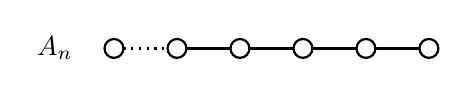
\begin{tikzpicture}[scale=.4]
    \draw (-1,0) node[anchor=east]  {$A_n$};
    \foreach \x in {0,...,5}
    \draw[xshift=\x cm,thick] (\x cm,0) circle (.3cm);
    \draw[dotted,thick] (0.3 cm,0) -- +(1.4 cm,0);
    \foreach \y in {1.15,...,4.15}
    \draw[xshift=\y cm,thick] (\y cm,0) -- +(1.4 cm,0);
  \end{tikzpicture}
\end{center}

There is a correspondence with each flag selecting one variety(?) to a generator, though it is not a bijection. (define before flag and find a word for variety)

The flag consists of a vertex, an edge containing the vertex, a 2-face containing the edge \ldots etc. If we focus on one variety, then the corresponding symmetry is the hyperplane $\rho $ that fixes the lower dimension varieties and keeps invariant the higher ones. (By keep invariant I mean the subspace goes to the same subspace, not necessarily point to point, while fix is point to point)

We will see it more clearly in the next subsection.

\subsection{Classification of Platonic Solids} (Probably cut this section idk)
There exist 5 platonic solids. We can think all the solids in the projective space to make easier computations.

\textbf{Tetrahedron $A_3$}

Vertices are the indicator vectors of $\binom{[4]}{1}$

We have a flag $\{V_1, V_2, V_3\}$, where $V_i$ are projective varieties that correspond to a vertex, edge and face respectively and for each  $V_i$ we have the induced hyperplane $\rho_i $ associated with the reflection $s_i$. If we compute the normal vectors of the planes:

 \[
\rho_1^\perp = \begin{pmatrix} 1\\-1\\0\\0 \end{pmatrix} , \quad
\rho_2^\perp = \begin{pmatrix} 0\\1\\-1\\0 \end{pmatrix} , \quad
\rho_3^\perp = \begin{pmatrix} 0\\0\\1\\-1 \end{pmatrix} \quad
\Rightarrow \quad
\angle \rho_1 \rho _2 = \frac{\pi}{3}, \quad
\angle \rho_1 \rho _3 = \frac{\pi}{2}, \quad
\angle \rho_2 \rho _3 = \frac{\pi}{3}
\] 
And then we deduce the diagram
\begin{tikzcd}
	{\textcircled{1}} & {\textcircled{2}} & {\textcircled{3}}
	\arrow[no head, from=1-1, to=1-2]
	\arrow[no head, from=1-2, to=1-3]
\end{tikzcd}

\textbf{Cube $B_3$}

\textbf{Octahedron $B_3$}

Vertices are the indicator vectors of $\binom{[4]}{2}$

We have a flag $\{V_1, V_2, V_3\}$, where $V_i$ are projective varieties that correspond to a vertex, edge and face respectively and for each  $V_i$ we have the induced hyperplane $\rho_i $ associated with the reflection $s_i$. If we compute the normal vectors of the planes:

 \[
\rho_1^\perp = \begin{pmatrix} 1\\-1\\0\\0 \end{pmatrix} , \quad
\rho_2^\perp = \begin{pmatrix} 1\\0\\-1\\0 \end{pmatrix} , \quad
\rho_3^\perp = \begin{pmatrix} 1\\1\\-1\\-1 \end{pmatrix} \quad
\Rightarrow \quad
\angle \rho_1 \rho _2 = \frac{\pi}{3}, \quad
\angle \rho_1 \rho _3 = \frac{\pi}{2}, \quad
\angle \rho_2 \rho _3 = \frac{\pi}{4}
\] 
And then we deduce the diagram
\begin{tikzcd}
	{\textcircled{1}} & {\textcircled{2}} & {\textcircled{3}}
	\arrow[no head, from=1-1, to=1-2]
	\arrow["4", no head, from=1-2, to=1-3]
\end{tikzcd}

\textbf{Dodecahedron $H_3$}

\textbf{Icosahedron $H_3$}


\section{Description of Coxeter Groups}
\subsection{Group $A_n$}
\begin{tikzcd}
	\circ & \circ & \cdots & \circ & \circ
	\arrow[from=1-1, to=1-2]
	\arrow[from=1-2, to=1-3]
	\arrow[from=1-3, to=1-4]
	\arrow[from=1-4, to=1-5]
\end{tikzcd}

We can think type $A_n$ Coxeter Groups as groups generated by the reflections  $s_1, \ldots, s_{n-1}$ whose associated hyperplanes are defined by
\[
\rho_1 ^\perp = \begin{pmatrix} 1 \\ -1 \\ 0\\ \vdots \\ 0 \end{pmatrix} , \quad 
\rho_2 ^\perp = \begin{pmatrix} 0 \\ 1 \\ -1\\ \vdots \\ 0 \end{pmatrix} , \quad \ldots \quad
\rho_{n-1} ^\perp = \begin{pmatrix} 0 \\ \vdots \\ 0 \\ 1\\ -1 \end{pmatrix} , \quad 
\] 
It is easy to see that the angles between the hyperplanes are
\[
\angle \rho_i \rho_{i+1} = \frac{\pi}{3}, \quad 
\angle \rho_i \rho _{j} = \frac{\pi}{2}\ if\ i-j\neq \pm 1 \quad 
\] 
so that corresponds to the Dynkin diagram, and thus to the Coxeter group


\subsection{Group $B_n$}
\begin{tikzcd}
	\circ & \circ & \cdots & \circ & \circ
	\arrow["4", from=1-1, to=1-2]
	\arrow[from=1-2, to=1-3]
	\arrow[from=1-3, to=1-4]
	\arrow[from=1-4, to=1-5]
\end{tikzcd}

We can think type $B_n$ Coxeter groups as the group generated by the reflections  $\tau, s_1, \ldots, s_n$, whose associated hyperplanes are defined by
\[
\rho_\tau ^\perp = \begin{pmatrix} 1 \\ 0 \\ 0 \\  \vdots \\ 0 \end{pmatrix} , \quad 
\rho_1 ^\perp = \begin{pmatrix} 1 \\ 1 \\ 0\\ \vdots \\ 0 \end{pmatrix} , \quad 
\rho_2 ^\perp = \begin{pmatrix} 0 \\ 1 \\ 1\\ \vdots \\ 0 \end{pmatrix} , \quad \ldots \quad
\rho_n ^\perp = \begin{pmatrix} 0 \\ \vdots \\ 0 \\ 1\\ 1 \end{pmatrix} , \quad 
\] 

One can check that the angles between the hyperplanes are
\[
\angle \rho_\tau \rho _1 = \frac{\pi}{4}, \quad 
\angle \rho_\tau \rho _i = \frac{\pi}{2}\  if\ i>1, \quad 
\angle \rho_i \rho _{i+1} = \frac{\pi}{3}, \quad 
\angle \rho_i \rho _{j} = \frac{\pi}{2}\ if\ i-j\neq \pm 1 \quad 
\] 
so the construction correspond to the Dynkin diagram, and thus to the coxeter group.

\subsection{Group $D_n$}
\begin{tikzcd}
	\circ \\
	& \circ & \circ & \cdots & \circ & \circ \\
	\circ
	\arrow[from=2-2, to=2-3]
	\arrow[from=2-3, to=2-4]
	\arrow[from=2-4, to=2-5]
	\arrow[from=1-1, to=2-2]
	\arrow[from=3-1, to=2-2]
	\arrow[from=2-5, to=2-6]
\end{tikzcd}

We can think type $D_n$ Coxeter groups as the group generated by the reflections  $\tau_1, \tau_2, s_1, \ldots, s_n$, whose associated hyperplanes are defined by
\[
\rho_{\tau_1} ^\perp = \begin{pmatrix} 1 \\ 1 \\ 0 \\  \vdots \\ 0 \end{pmatrix} , \quad 
\rho_{\tau_2} ^\perp = \begin{pmatrix} -1 \\ 1 \\ 0\\ \vdots \\ 0 \end{pmatrix} , \quad 
\rho_1 ^\perp = \begin{pmatrix} 0 \\ 1 \\ 1\\ \vdots \\ 0 \end{pmatrix} , \quad \ldots \quad
\rho_n ^\perp = \begin{pmatrix} 0 \\ \vdots \\ 0 \\ 1\\ 1 \end{pmatrix} , \quad 
\] 

One can check that the angles between the hyperplanes are
\[
\angle \rho_{\tau_1} \rho _{\tau _2} = \frac{\pi}{2}, \quad
\angle \rho_{\tau_1} \rho _{1} = \frac{\pi}{3}, \quad
\angle \rho_{\tau_2} \rho _{1} = \frac{\pi}{3}, \quad
\angle \rho_i \rho _{i+1} = \frac{\pi}{3}, \quad 
\angle \rho_i \rho _{j} = \frac{\pi}{2}\ if\ i-j\neq \pm 1 \quad 
\] 
so the construction correspond to the Dynkin diagram, and thus to the coxeter group.


\section{Regular Subdivision and height functions}
\subsection{Hypersymplex $\Delta(k, n)$}
Given a set of points $T$, we define a height function as  $h:T \to \mathbb{R}$.

A subset $S$ of points is a (lower) regular subdivision induced by $h$ if the convex hull of $S$ is described by the lower convex hull of the polytope $T\times h(T)$ (not well explained)

The height function $h$ is said to be \textit{M-convex} if the regular subdivision induced by $h$ is permutahedral.

We will use the notation $Sij := S\cup \{i\}\cup \{j\}$

\begin{definition}[3-Term Plücker Relations] Let $h $ be a height function on $\Delta(d, n)$.
We say that 3TPR holds if for each $S\in \binom{[n]}{ d-2}$ and $i, j, k, l \not\in S$, the minimum
\[
\min \Big\{h(Sij) + h(Skl), \ h(Sik) + h(Sjl),\  h(Sil) +  h(Sjl)\Big\}
\] 
is attained at least twice.
\end{definition}

\begin{theorem}[] A height function induces a permutahedral regular division if the \textbf{3-Term Plücker Relations} (3TPR) holds.
\end{theorem}

\begin{proof}
We fix $S$ and we abbreviate $h_{ij} = h(Sij)$.

Suppose the 3TPR holds. Given the height function $h$ we fix a linear functional $\varphi = (\varphi _1, \ldots, \varphi _n, \varphi _{n+1})$ with $\varphi _{n+1}>0$ such that the set of vertices induced by $Q\subseteq \Delta(d, n)$ given by
\[
Q = \{A\in \Delta(d, n) : \varphi (A, h(A)) \text{ is minimum}\}
\] 
We now can relabel the indices of the elements of $Q$ and $\varphi $ removing all the terms that are $1$ or zero always (when applying the functional the result is the same inside $Q$) and relabeling the remaining from $1$ to  $m$.

In the cases $m = 2$ and  $m=3$ one can check the subpolytope $Q$ permutahedral. For case $m\ge 4$ we pick 4 indices $i, j, k, l$ of elements of $Q$ and $\varphi $. 

We can assume without loss of generality that $Sij, Skl \in Q$ now we want to prove that exchange axiom is satisfied: i.e. whithout loss of generality $Sik, Sjl\in Q$.

We can express the 3TPR in the following way:
\[
  3TPR \iff h_{ij} + h_{kl} = h_{ik} + h_{jl}\le h_{il} + h_{jk}
\] 

The condition for $Sij, Skl$ to lie in a regular subdivision is that
\[
\varphi _i + \varphi _j + \varphi _{n+1} h_{ij} = 
\varphi _k + \varphi _l + \varphi _{n+1} h_{kl} \le 
\begin{cases}
  \varphi _i + \varphi _k + \varphi _{n+1}h_{ik}\ \  (1)\\
  \varphi _j + \varphi _l + \varphi _{n+1}h_{jl} \ \   (2)
\end{cases}
\] 
This leads to the equations
\begin{align*}
 \varphi _j - \varphi _k \le \varphi _{n+1}(h_{ik}-h_{ij})  \\
 \varphi _i - \varphi _l \le \varphi _{n+1}(h_{lj}-h_{ij})  \\
 \varphi _l - \varphi _i \le \varphi _{n+1}(h_{ik}-h_{kl})  \\
 \varphi _k - \varphi _j \le \varphi _{n+1}(h_{jl}-h_{kl})
\end{align*}
Summing up the equations we get
\[
0\le 2\varphi_{n+1}(h_{ik}+ h_{jl} - h_{ij}-h_{kl}) \Rightarrow h_{ij} + h_{kl} \le h_{ik} + h_{jl}
\] 
But this inequality should be an equality under the assumption of 3TPR, so all the above inequalities should be equalities, and (1) and (2) imply $Sik, Sjl\in Q$
\end{proof}



\subsection{Hypercube $\square_n$}

Now we switch from type $A_n$ coxeter groups to type $B_n$

\begin{definition}[Hypercube]
$\square_n  = conv\{x\in \mathbb{R}^n: x_i = \pm 1\}$
\end{definition}

We notice the following injection, labeling the indices of $\Delta(n, 2n)$ as  $-n, -n+1,  \ldots -1, 1, 2, \ldots ,n$: (explain more)
\begin{align*}
  V(\square_n) &\to V(\Delta(n, 2n)) \\
  x_i = 1 & \mapsto y_i=1, y_{-i}=0 \\
  x_i = -1 & \mapsto y_{-i}=1, y_{i}=0 \\
\end{align*}

If we restrict the posible values of the vertices of $\Delta(n, 2n)$ such that they fulfill $y_i + y_{-i} = 1$ we get the bijection
\[
\square_n \cong \Delta(n, 2n) |_{y_i+y_{-i}=1}
\] 

\begin{observation}
  \label{obs1}
  Edges parallel to $e_j$ in  $\square_n$ $\iff$ edges parallel to $e_j-e_{-j}$ in $\Delta(n, 2n)$
\end{observation}

\begin{definition}[Cubohedron]
The cubohedron is the convex hull of a subset of vertices of the hypercube $C\subseteq \square_n$ whose edges are parallel to $e_j$
\end{definition}

We now want to find a relation similar to 3TPR in the case of  Coxeter groups of type $B_n$.

Since the edges of $C$ are be identified with the vertices of a subset $P\subseteq \Delta(n, 2n)$, and the edges of this subset are parallel to $e_j-e_{-j}$ by the observation, then $P$ is permutahedral.

Now we consider a height function on $h:\square_n \to \mathbb{R}$ which we can identify as a height funcion $h': \bigslant{\Delta(n, 2n)}{y_i+i_{-i} = 1}$. Thus, we can apply 3TPR to 

\textbf{Notation:} Given a height function $h$, we say $h_{i-j}:=h(Ti-j)$, where $Ti-j$ is the element $T$ such that $x_i = 1, x_j = -1$.

\begin{definition}[New Relations] Let $h$ be an height function on $\square_n$.
We say that New Relations (NR) holds if for each $T\in \binom{[n]}{d-2}$ and $i, j$
\[
h(Tij)+ h(T-i-j) = h(T-ij) + h(Ti-j)
\] 
\end{definition}
\begin{theorem}[] A height function induces a cubohedral regular division if the \textbf{New Relations} (NR) hold.
\end{theorem}

\begin{proof}
  
Suppose NR holds. Given the height function $h$ we fix a linear functional  $\varphi = (\varphi _1, \ldots, \varphi _n, \varphi _{n+1})$ with $\varphi _{n+1}>0$ such that the vertices of the regular division polytope $C\in \square_n$ is given by
\[
C = \{A \in M: \varphi (A, h(A)) \text{ is minimum}\}
\] 
We now can relabel the indices of the elements of $C$ and $\varphi $ removing all the terms that are the same in all vectors and relabeling the remaining from 1 to $m$.

If  $m = 1$ the result is trivially cubohedral (1 point). If  $m\ge 2$ we can pick two indices $i, j$ and assume without loss of generality  $T_{ij}, T_{-i-j}\in A$. Now out work is to proof that $T_{i-j}, T_{-ij} \in A$.

The conditions for $T_{ij}, T_{-i-j}$ to lie in the regular subdivision is that 
\[
\varphi _i + \varphi _j + \varphi _{n+1}h_{ij} = -\varphi _i -\varphi _j + \varphi _{n+1}h_{-i-j} \le \begin{cases}
  \varphi _i -\varphi _j + \varphi _{n+1}h_{i-j} \\
  -\varphi _i + \varphi _j + \varphi _{n+1}h_{-ij}
\end{cases}
\] 
This leads to the equations
\begin{align*}
  2\varphi _j\le \varphi _{n+1}(h_{i-j}- h_{ij}) \\
  2\varphi _i\le \varphi _{n+1}(h_{-ij}- h_{ij}) \\
  -2\varphi _i\le \varphi _{n+1}(h_{i-j}- h_{-i-j}) \\
  -2\varphi _j\le \varphi _{n+1}(h_{-ij}- h_{-i-j})
.\end{align*}
Summing up the equations we get
\[
0\le 2\varphi_{n+1}(h_{i-j} + h_{-ij}-h_{ij}-h_{-i-j}) \Rightarrow h_{ij} + h_{-i-j} \le h_{i-j} + h_{-ij}
\] 
But this inequality should be an equality by NR, so all the inequalities before must be equalities, meaning $T_{i-j}, T_{-ij}\in A$ 

\end{proof}




\end{document}





















